\subsection{ROC curve}
The ROC (Receiver Operating Characteristics) curve is a plot which shows the performance of a binary classifier as its discrimination threshold is varied.\\
The curve is created by plotting the true positive rate vs the false positive rate at various threshold settings.

\subsection{ROC plot of trained models}
Below is the ROC plot of all the trained models.
\begin{center}
    \captionsetup{type=figure}
    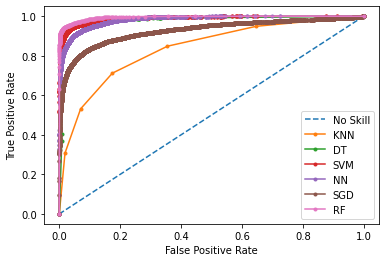
\includegraphics[width=250px]{AUC.png}
    \captionof{figure}{ROC Curve of all trained models}
\end{center}

The AUC (Area Under Curve) for each model was calculated to be 
\begin{itemize}
    \item KNN=0.837
    \item DT=0.981
    \item SVM=0.988
    \item NN=0.982
    \item SGD=0.927
    \item RF=0.995
\end{itemize}





